\documentclass[11pt,a4paper]{scrarticle}
\usepackage[utf8]{inputenc}
\usepackage{cmap}
\usepackage[T2A]{fontenc}
\usepackage[russian]{babel}
\usepackage{amsmath,amssymb,amsthm,mathtools}
\usepackage{array}

\usepackage{indentfirst}
\usepackage{xcolor,graphicx, tikz, wrapfig}
\usepackage{longtable}

% \usepackage{minted}
% \usemintedstyle{vs}

\usepackage[left=2cm,right=2cm,top=2cm,bottom=2cm,bindingoffset=0cm]{geometry}

\usepackage[unicode]{hyperref}
\definecolor{linkcolor}{HTML}{0000E6}
\definecolor{urlcolor}{HTML}{0000E6}
\definecolor{citecolor}{HTML}{0000E6}
\hypersetup{pdfpagemode=None,linktoc=page,citecolor=citecolor,linkcolor=linkcolor,urlcolor=urlcolor,colorlinks=true}

\theoremstyle{definition}
\newtheorem{subtask}{Пункт}

\DeclareMathOperator*{\argmax}{arg\,max}
\DeclareMathOperator*{\argmin}{arg\,min}
\newcommand{\floor}[1]{\left\lfloor #1 \right\rfloor}
\newcommand{\ceil}[1]{\left\lceil #1 \right\rceil}


\setlength{\parindent}{1cm}

\author{Клычков Максим Дмитриевич}

\begin{document}

\centerline{\textbf{\huge Алгоритмы и структуры данных-1}}
\centerline{\textbf{SET 2. Задача A1.}}
\begin{flushright}
	\emph{Осень 2024. Клычков М. Д.}
\end{flushright}

\begin{figure}[htp]
	\centering
	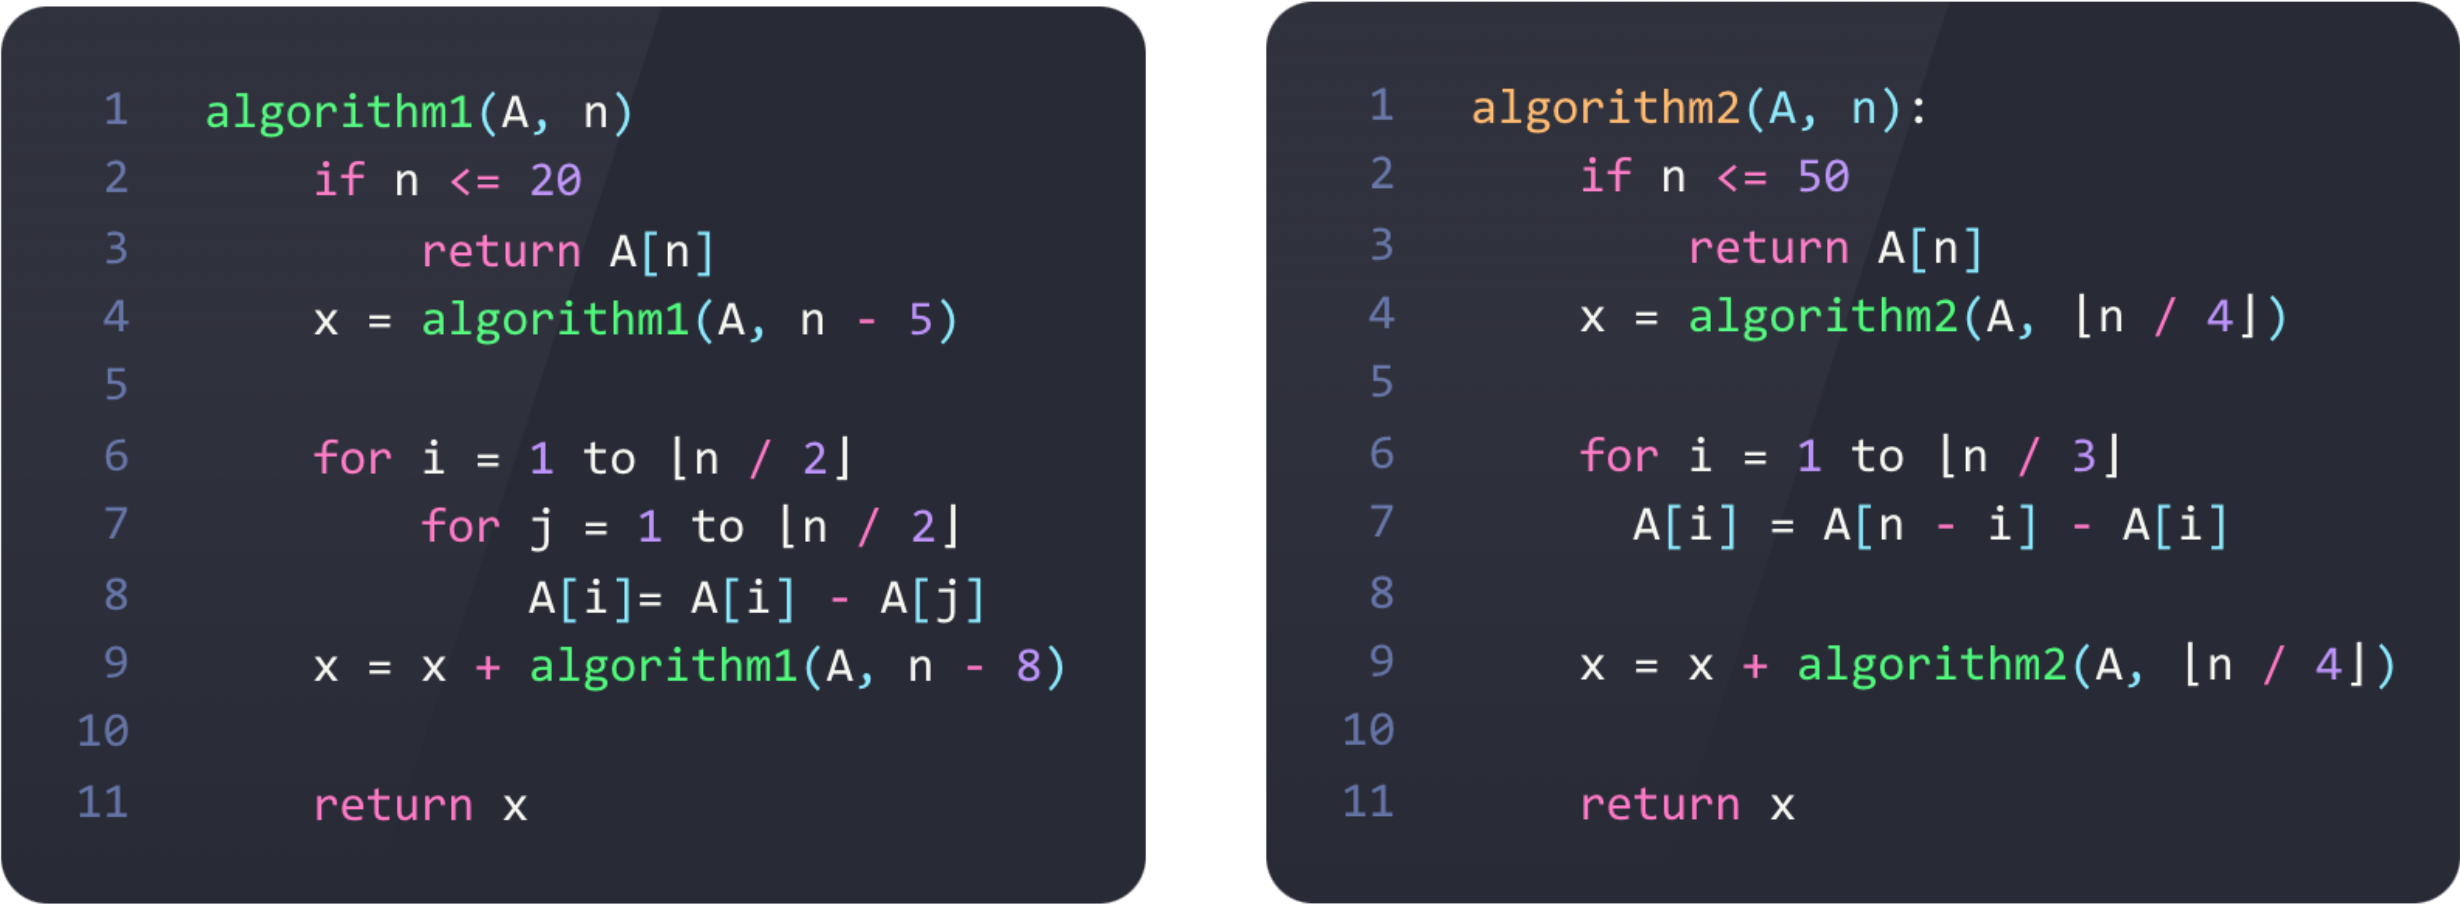
\includegraphics[width=\textwidth]{code.png}
\end{figure}

\begin{subtask}
	Проанализируем первый алгоритм. В рекурсивную ветку вычислений входят вызовы функции \texttt{algorithm1} на $4$ и $9$ строках кода, причем аргументы передаются разные.
	В нерекурсивной ветке вычислений, учитывая, что все арифметические операции выполняются за константное время, производится $\Theta\left(\floor{\frac{n}{2}}^2\right) + \Theta(1) = \Theta\left(\left(\frac{n}{2}\right)^2\right) = \Theta(n^2)$ операций. Такое количество обеспечивается вложенным циклом от $1$ до $\floor{\frac{n}{2}}$ каждый.
	Также необходимо учесть, что при $n \leq 20$ алгоритм будет работать за $\Theta(1)$.

	Можно еще заметить, что на каждом шаге рекурсии происходит копирование массива $A$. Не понятно, является ли это одним из допущений псевдокода или задуманным копированием, но в любом случае нерекурсивная ветка даже с учетом копирования: $\Theta(n^2) + \Theta(n) = \Theta(n^2)$

	\begin{equation}
		\label{eqn:t1}
		T_1(n) = \begin{dcases}
			\Theta(1)                             & , n \leq 20 \\
			T_1(n - 5) + T_1(n - 8) + \Theta(n^2) & , n > 20
		\end{dcases}
	\end{equation}

	Проанализируем второй алгоритм. В рекурсивную ветку вычислений входят вызовы функции \texttt{algorithm2} на $4$ и $9$ строках кода, аргументы передаются одинаковые.
	В нерекурсивной ветке вычислений, учитывая, что все арифметические операции выполняются за константное время, производится $\Theta\left(\floor{\frac{n}{3}}\right) + \Theta(1) = \Theta\left(\frac{n}{3}\right) = \Theta(n)$ операций. Такое количество обеспечивается циклом от $1$ до $\floor{\frac{n}{3}}$.

	Будем считать, что $n$ принимает значения равные степеням четверки, это допущение позволит нам избавиться от округления вниз и в то же время никак не повлияет на асимптотическую оценку.
	Также необходимо учесть, что при $n \leq 50$ алгоритм будет работать за $\Theta(1)$.
	Аналогично первому алгоритму тут уместна оговорка о копировании массива.

	\begin{equation}
		\label{eqn:t2}
		T_2(n) = \begin{dcases}
			\Theta(1)                                & , n \leq 50 \\
			2T_2\left(\frac{n}{4}\right) + \Theta(n) & , n > 50
		\end{dcases}
	\end{equation}
\end{subtask}

\begin{subtask}
	Разберем сначала \textbf{первый} алгоритм. Планируется сначала сделать предположение, затем доказать его при помощи метода подстановки. Нас интересует рассмотрение только случая $n > 20$ из двух возможных \eqref{eqn:t1}.

	Так как функция $T_1(n)$ монотонно возрастающая, верно, что
	\begin{align}
		\label{eqn:t1leq} T_1(n) & = T_1(n - 5) + T_1(n - 8) + \Theta(n^2) \leq 2 T_1(n - 5) + \Theta(n^2) \\
		\label{eqn:t1geq} T_1(n) & = T_1(n - 5) + T_1(n - 8) + \Theta(n^2) \geq 2 T_1(n - 8) + \Theta(n^2)
	\end{align}

	Обозначим $T_1^1(n) = 2 T_1^1(n - 8) + \Theta(n^2)$ и $T_1^2(n) = 2 T_1^2(n - 5) + \Theta(n^2)$. Тогда можем записать следующее двойное неравенство:

	$$
		T_1^1(n) \leq T_1(n) \leq T_1^2(n)
	$$

	Нашей целью является оценка верхней и нижней асимптотической грани, поэтому можно найти функции $f(n)$ и $g(n)$ такие, что $T_1^1(n) = \Omega(f(n))$ и $T_1^2(n) = O(g(n))$, тогда, пользуясь неравенством, можно получить, что $T_1(n) = \Omega(f(n))$ и $T_1(n) = O(g(n))$.

	\begin{enumerate}
		\item Гипотеза $T_1^1(n) = 2 T_1^1(n - 8) + \Theta(n^2) = \Omega(2^\frac{n}{8})$, а именно $T_1^1(n) \geq c 2^\frac{n}{8}$.
		      Тогда, пользуясь $T_1^1(n - 8) \geq c 2^\frac{n - 8}{8}$, делаем подстановку:
		      \begin{align*}
			      T_1^1(n) & \geq 2 \cdot c 2^\frac{n - 8}{8} + qn^2 \\
			               & = c \cdot 2^\frac{n}{8} + qn^2
		      \end{align*}

		      \begin{align*}
			      c \cdot 2^\frac{n}{8} + qn^2 & \geq c \cdot 2^\frac{n}{8} \\
			      qn^2                         & \geq 0
		      \end{align*}
		      Пусть $c = 1, n_0 = 1, q > 0$, получаем верное утверждение $\blacksquare$

		\item Гипотеза $T_1^2(n) = 2 T_1^2(n - 5) + \Theta(n^2) = O(2^\frac{n}{5}n^2)$, а именно $T_1^2(n) \leq c \cdot 2^\frac{n}{5} \cdot n^2 - d \cdot 2^\frac{n}{5} \cdot n - p \cdot 2^\frac{n}{5}$.
		      Тогда, пользуясь $T_1^2(n - 5) \leq c \cdot 2^\frac{n - 5}{5} \cdot (n-5)^2 - d \cdot 2^\frac{n - 5}{5} \cdot (n - 5) - p \cdot 2^\frac{n - 5}{5}$, делаем подстановку.
		      \begin{align*}
			      T_1^2(n) & \leq 2 c \cdot 2^\frac{n - 5}{5} \cdot (n-5)^2 - 2 d \cdot 2^\frac{n - 5}{5} \cdot (n - 5) - 2 p \cdot 2^\frac{n - 5}{5} + qn^2 \\
			               & = c \cdot 2^\frac{n}{5} n^2 - (10c + d) \cdot 2^\frac{n}{5} n - (25c - 5d + p) \cdot 2^\frac{n}{5} + qn^2
		      \end{align*}

		      \begin{align*}
			      c \cdot 2^\frac{n}{5} n^2 - (10c + d) \cdot 2^\frac{n}{5} n - (25c - 5d + p) \cdot 2^\frac{n}{5} + qn^2 & \leq c \cdot 2^\frac{n}{5} \cdot n^2 - d \cdot 2^\frac{n}{5} \cdot n - p \cdot 2^\frac{n}{5} \\
			      -10c \cdot 2^\frac{n}{5} n - (25 c - 5d) 2^\frac{n}{5} + qn^2                                           & \leq 0
		      \end{align*}

		      Пусть $c = 1, d = 5$, тогда получим
		      \begin{align*}
			      10 \cdot 2^\frac{n}{5} n \geq mn^2 \\
			      10 \cdot 2^\frac{n}{5} \geq mn
		      \end{align*}

		      Очевидно, что на бесконечности это верно $\blacksquare$
	\end{enumerate}
	$$
		T_1^1(n) = \Omega(2^\frac{n}{8}) \wedge T_1^2(n) = O(2^\frac{n}{5}n^2) \Rightarrow T_1(n) = \Omega(2^\frac{n}{8}) \wedge T_1(n) = O(2^\frac{n}{5}n^2)
	$$
	\pagebreak

	Разберем \textbf{второй} алгоритм. Докажем, что $T_2(n) = \Theta(n)$. Для этого применим метод подстановки два раза:

	\begin{enumerate}
		\item Гипотеза $T_2(n) = O(n) \Leftrightarrow T_2(n) \leq cn$. Тогда, пользуясь
		      $T_2\left(\frac{n}{4}\right) \leq \frac{cn}{4}$, делаем подстановку:
		      \begin{align*}
			      T_2(n) & \leq 2 \cdot \frac{cn}{4} + dn           \\
			             & = \frac{cn}{2} + dn                      \\
			             & = \left(\frac{c}{2} + d\right) n \leq cn
		      \end{align*}

		      $d$ фиксированная положительная константа, найдем для нее подходящее $c$.
		      Например, при $c = 4d$: $\left(\frac{4d}{2} + d\right) n \leq 4dn \Leftrightarrow 3d n \leq 4d n$, что верно $\forall n \geq 1$ $\blacksquare$
		\item Гипотеза $T_2(n) = \Omega(n) \Leftrightarrow T_2(n) \geq cn$. Тогда, пользуясь
		      $T_2\left(\frac{n}{4}\right) \geq \frac{cn}{4}$, делаем подстановку:
		      \begin{align*}
			      T_2(n) & \geq 2 \cdot \frac{cn}{4} + dn           \\
			             & = \frac{cn}{2} + dn                      \\
			             & = \left(\frac{c}{2} + d\right) n \geq cn
		      \end{align*}
		      $d$ фиксированная положительная константа, найдем для нее подходящее $c$.
		      Например, при $c = d$: $\left(\frac{d}{2} + d\right) n \geq dn \Leftrightarrow 1.5d n \geq d n$, что верно $\forall n \geq 1$ $\blacksquare$
	\end{enumerate}

	$$
		T_2(n) = O(n) \land T_2(n) = \Omega(n) \Longrightarrow T_2(n) = \Theta(n)
	$$
\end{subtask}

\end{document}